%==============================================================================
%== template for LATEX poster =================================================
%==============================================================================
%
%--A0 beamer slide-------------------------------------------------------------
\documentclass[final]{beamer} % use beamer
%\usepackage{program} %causing issues with compile
\usepackage{algorithmic} %sudo code
\usepackage{algorithm}  %more sudo code
\usepackage[orientation=portrait,
		size=custom, width=55.8, height=91.4,  % poster size 22in=55.88cm 91.44cm=36in
		scale=.99         % font scale factor
	]{beamerposter}    % beamer in poster size

\usepackage{listings}
%--some needed packages--------------------------------------------------------
\usepackage[american]{babel}  % language 
\usepackage[utf8]{inputenc}   % std linux encoding



%
%==The poster style============================================================
\usetheme{pgassc11poster}            % our poster style
%--set colors for blocks (without frame)---------------------------------------
\setbeamercolor{block title}{fg=ngreen,bg=white}
\setbeamercolor{block body}{fg=black,bg=white}
%--set colors for alerted blocks (with frame)----------------------------------
%--textcolor = fg, backgroundcolor = bg, dblue is the jacobs blue
\setbeamercolor{block alerted title}{fg=white,bg=dblue!70}%frame color
\setbeamercolor{block alerted body}{fg=black,bg=dblue!10}%body color
%
%==Titel, date and authors of the poster=======================================
\title{Alternative High Performance Benchmarks}
\author{Kurt Rudolph, Vivek Kale, Lawrence C. Angrave, William D. Gropp}
\institute{Department of Computer Science, University of Illinois Urbana-Champaign}
\date{\today}
%
%==some usefull qm commands====================================================
%  |x>
\newcommand{\ket}[1]{\left\vert#1\right\rangle}
%  <x|
\newcommand{\bra}[1]{\left\langle#1\right\vert}
%  <x|y>
\newcommand{\braket}[2]{\left< #1 \vphantom{#2}\, \right\vert\left.\!\vphantom{#1} #2 \right>}
%  <x|a|y>
\newcommand{\sandwich}[3]{\left< #1 \vphantom{#2 #3} \right #2 \left|\vphantom{#1 #2} #3 \right>}
%  d/dt
\newcommand{\ddt}{\frac{d}{dt}}
%  D/Dx
\newcommand{\pdd}[1]{\frac{\partial}{\partial#1}}
%  |x|
\newcommand{\abs}[1]{\left\vert#1\right\vert}
%  k_{x}
\newcommand{\kv}[1]{\mathbf{k}_{#1}}




\begin{document}
	\begin{frame}[t]
		\begin{columns}[t] 
			  \begin{column}{0.60\paperwidth} 
%=======================Avstract======================================================================================
				\begin{alertblock}{Abstract}
					Benchmarks for High-Performance clusters generally focus on floating-point intensive calculations. Few of these address data intensive graph operations, a class of computation rapidly growing in demand.  As an alternative to standard floating-point benchmarks, a new benchmark, the Graph 500 has been proposed. The benchmark employ's multiple implementations with the intention to identify desecrate performance aspects via the comparative results, however a PGAS model has yet to be developed. This project focuses on understanding what capabilities a UPC Graph 500 implementation may offer. Specifically: 1. the UPC expressibility for irregular graph operations of Graph 500 and 2. simple performance testing of the efficiency of UPC.
				\end{alertblock}
				\vskip2ex
%=======================Linked List Traversal======================================================================================
				\begin{block}{Random Access}
					When performing graph operations, random access to memory and random process communication are generally very common.  This test looks at how well a UPC Graph 500 implementation of may handle these operations.  To do so, we implement a dot product employing randomized access and communication through the RDMA. 
				\end{block}
				\begin{columns}[t,totalwidth=0.60\paperwidth]
					\begin{column}{0.28\paperwidth}
						\lstinputlisting[language=C, basicstyle=\footnotesize]{ mpiSimpleSample.c}
					\end{column}
					\begin{column}{0.28\paperwidth}
						\begin{columns}[t,totalwidth=0.28\paperwidth]
							\begin{column}{0.12\paperwidth}
								\begin{center} 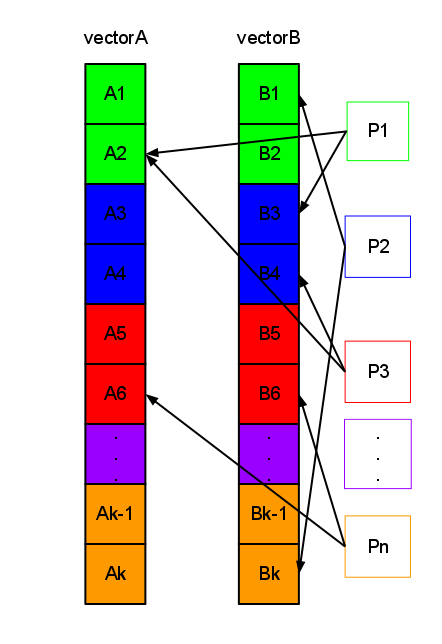
\includegraphics[width=0.12\paperwidth]{img/rand_access} \end{center}
							\end{column}
							\begin{column}{0.12\paperwidth}
								\begin{center} 
\includegraphics[width=0.12\paperwidth]{img/logo_graph500} \end{center}
							\end{column}
						\end{columns}
					\end{column}
				\end{columns}
				\vskip1ex
%A UPC thread t_i first chooses a random cell in v1 that belongs to it:   v1[rand()%n];   
%A UPC thread t_i then chooses a random cell in v2 to multiply with:    v2[rand()%n];  

%There is 1/p chance that a thread will access its own partition. There is (p-1)/p chance that a thread will have to go through the RDMA to retrieve the data it needs to do the floating-point multiplication.

%Other variants exist:  

%  - each thread runs through its own partition v1[(n/p)*i]  to v1[(n/p)*i] ,  and for each choose  v2[rand()%(n/p) + (n/p)*i] based on thread partition each thread has.

 %  - each thread chooses a random cell in its partition  of v1  and then chooses a cell in its partition of v2. 
  
 % - choose whether you want to have distinct pairs, or have some cells  repeated across pairs, or entire pairs repeated. 


%These tests can be representative of graph traversal operations and irregular algorithms. They particularly test the class of computation UPC one-sided programming model would be used for. 
%=======================Linked List Traversal======================================================================================
				\begin{block}{Linked List Traversal}
					As a simple test to measure the efficiency of UPC when performing graph operations, various linked list structure have been set and up an the linked list traversal of which is timed.  
				\end{block}
				\begin{columns}[t,totalwidth=0.60\paperwidth]
					\begin{column}{0.28\paperwidth}
						\begin{center} \bf{Sequential Node, Sequential Process} \end{center}
						\begin{columns}[t,totalwidth=0.28\paperwidth]
							\begin{column}{0.12\paperwidth}
								\begin{center} 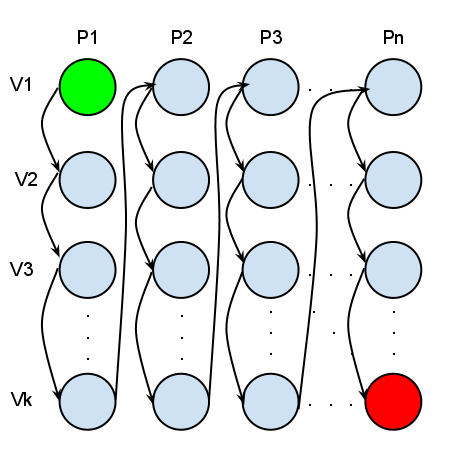
\includegraphics[width=0.12\paperwidth]{img/linked_list/seq_node_seq_proc} \end{center}
							\end{column}
							\begin{column}{0.12\paperwidth}
								\begin{center} 
\includegraphics[width=0.12\paperwidth]{img/logo_graph500} \end{center}
							\end{column}
						\end{columns}
					\end{column}
					\begin{column}{0.28\paperwidth}
						\begin{center} \bf{Sequential Process, Sequential Node} \end{center}
						\begin{columns}[t,totalwidth=0.28\paperwidth]
							\begin{column}{0.12\paperwidth}
								\begin{center} 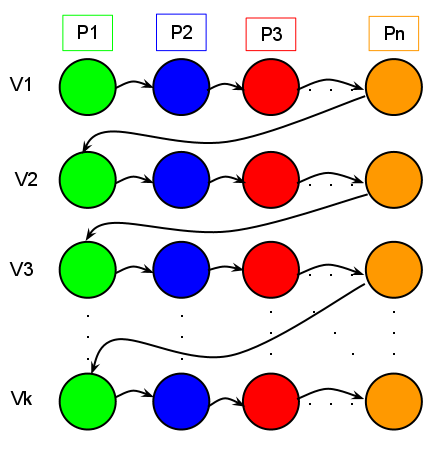
\includegraphics[width=0.12\paperwidth]{img/linked_list/seq_proc_seq_node} \end{center}
							\end{column}
							\begin{column}{0.12\paperwidth}
								\begin{center} 
\includegraphics[width=0.12\paperwidth]{img/logo_graph500} \end{center}
							\end{column}
						\end{columns}
					\end{column}
				\end{columns}
				\begin{columns}[t,totalwidth=0.60\paperwidth]
					\begin{column}{0.28\paperwidth}
						\begin{center} \bf{Random Node, Sequential Process} \end{center}
						\begin{columns}[t,totalwidth=0.28\paperwidth]
							\begin{column}{0.12\paperwidth}
								\begin{center} 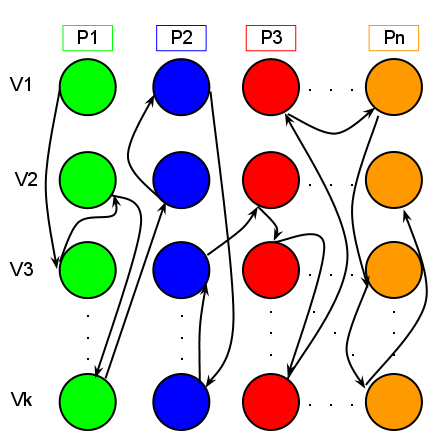
\includegraphics[width=0.12\paperwidth]{img/linked_list/rand_node_seq_proc} \end{center}
							\end{column}
							\begin{column}{0.12\paperwidth}
								\begin{center} 
\includegraphics[width=0.12\paperwidth]{img/logo_graph500} \end{center}
							\end{column}
						\end{columns}
					\end{column}
					\begin{column}{0.28\paperwidth}
						\begin{center} \bf{Sequential Process, Random Node} \end{center}
						\begin{columns}[t,totalwidth=0.28\paperwidth]
							\begin{column}{0.12\paperwidth}
								\begin{center} 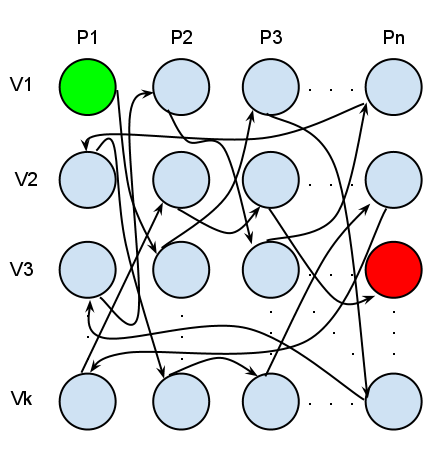
\includegraphics[width=0.12\paperwidth]{img/linked_list/seq_proc_rand_node} \end{center}
							\end{column}
							\begin{column}{0.12\paperwidth}
								\begin{center} 
\includegraphics[width=0.12\paperwidth]{img/logo_graph500} \end{center}
							\end{column}
						\end{columns}
					\end{column}
				\end{columns}
				\begin{columns}[t,totalwidth=0.60\paperwidth]
					\begin{column}{0.28\paperwidth}
						\begin{center} \bf{Sequential Node, Random Process} \end{center}
						\begin{columns}[t,totalwidth=0.28\paperwidth]
							\begin{column}{0.12\paperwidth}
								\begin{center} 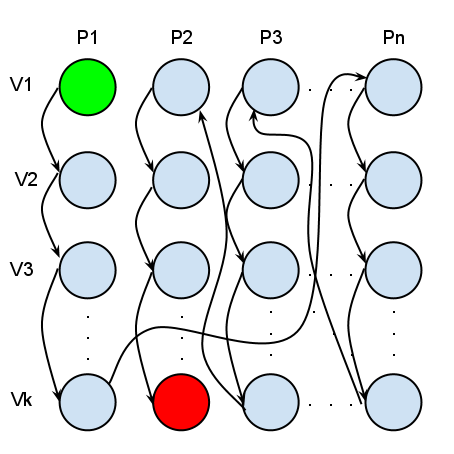
\includegraphics[width=0.12\paperwidth]{img/linked_list/seq_node_rand_proc} \end{center}
							\end{column}
							\begin{column}{0.12\paperwidth}
								\begin{center} 
\includegraphics[width=0.12\paperwidth]{img/logo_graph500} \end{center}
							\end{column}
						\end{columns}
					\end{column}
					\begin{column}{0.28\paperwidth}
						\begin{center} \bf{Random Process, Sequential Node} \end{center}
						\begin{columns}[t,totalwidth=0.28\paperwidth]
							\begin{column}{0.12\paperwidth}
								\begin{center} 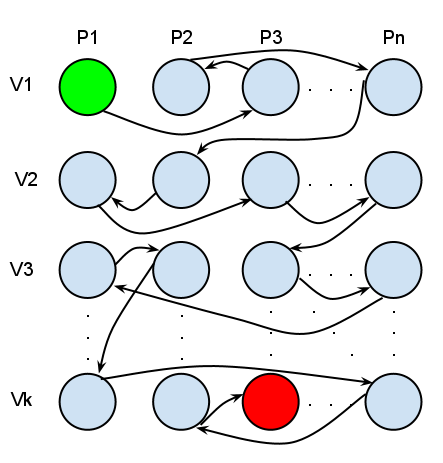
\includegraphics[width=0.12\paperwidth]{img/linked_list/rand_proc_seq_node} \end{center}
							\end{column}
							\begin{column}{0.12\paperwidth}
								\begin{center} 
\includegraphics[width=0.12\paperwidth]{img/logo_graph500} \end{center}
							\end{column}
						\end{columns}
					\end{column}
				\end{columns}
				\begin{columns}[t,totalwidth=0.60\paperwidth]
					\begin{column}{0.28\paperwidth}
						\begin{center} \bf{Random Node, Random Process} \end{center}
						\begin{columns}[t,totalwidth=0.28\paperwidth]
							\begin{column}{0.12\paperwidth}
								\begin{center} 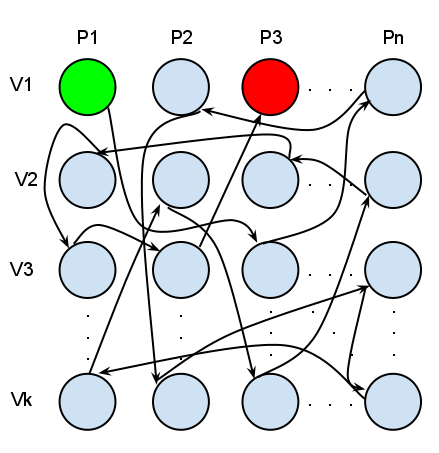
\includegraphics[width=0.12\paperwidth]{img/linked_list/rand_proc_rand_node} \end{center}
							\end{column}
							\begin{column}{0.12\paperwidth}
								\begin{center} 
\includegraphics[width=0.12\paperwidth]{img/logo_graph500} \end{center}
							\end{column}
						\end{columns}
					\end{column}
					\begin{column}{0.28\paperwidth}
						Discussion of the results...........................................................
					\end{column}
				\end{columns}
%=======================Multi Process Linked List Traversal======================================================================================
			\end{column}
%===rightcolumn=================================================================
  \begin{column}{0.28\paperwidth}% the right size for a 3-column layout
%--requirements block-----------------------------------------------------------
   \begin{block}{Discussion of all Results}
       Since the beamer package is used, basically all latexbeamer functions are
    supported \cite{beamerdoc}. The \emph{cpbgposter} style comes with some
    special features:
    \vskip1ex
    \begin{itemize}
     \item {\bf Poster Frame}\\
      A {\color{dblue}jacobs university blue} frame surrounding the whole poster
      and the title is drawn automatically\\\vskip1ex
     \item {\bf Poster Title}\\
      The title, authors, institute and the jub logo are placed automatically
      at the top of the poster. You can define them easily with the commands:
      \begin{semiverbatim}%\verb does not work with beamer
       {\color{red}\\title}\{...\}\newline
       {\color{red}\\author}\{...\}\newline
       {\color{red}\\institute}\{...\}
      \end{semiverbatim}
      The frame around the Title is also adjusted automatically to fit the
      number of lines in the title\\ \vskip1ex
     \item {\bf Blocks}\\
      Up to now there are two different block environment.
      The standard block:
      \begin{semiverbatim}
       {\color{red}\\begin}\{{\color{blue}block}\}\{Caption\}\newline
       \hskip1ex.......\newline
       {\color{red}\\end}\{{\color{blue}block}\}
      \end{semiverbatim}
      This creates a block with justified text and a fancy underlined green
      title. And then there is the alerted block:
      \begin{semiverbatim}
       {\color{red}\\begin}\{{\color{blue}alertblock}\}\{Caption\}\newline
       \hskip1ex.......\newline
       {\color{red}\\end}\{{\color{blue}alertblock}\}
      \end{semiverbatim}
      With this environment you can create a nicely framed block.\\\vskip1ex
      \item {\bf Bibliography}\\
      The default beamer bibliography style was also tweaked so that you can use
      the standard bibliography commands.
      \begin{semiverbatim}
       {\color{red}\\begin}{\color{blue}\{thebibliography\}}\{\#\}\newline
       environment contents\newline
       {\color{red}\\end}{\color{blue}\{thebibliography\}}
      \end{semiverbatim}
    \end{itemize}
   \end{block}

%--features block---------------------------------------------------------------
   \begin{block}{Conclusion and Future Work}
   \vskip1ex
    To compile you poster a current version the following a packages are 
    required
    \vskip1ex
    \begin{itemize}
     \item latexbeamer
     \item pgf (Tikz)
     \item beamerposter
    \end{itemize}
    \vskip1ex
    All those packages are contained in the TexLive distribution, which is
    also installed on our office computers. They should also be available in
    MikTeX if you have to work on a windows machine.
   \end{block}
   \vskip2ex
%--Remarks block----------------------------------------------------------------
   \begin{block}{Remarks}
    \begin{itemize}
     \item There are some warning messages due to the large font scaling.
      Ignore them!
     \item Sometimes the borders and frames look weird after compiling.
      Compile again, and it will be fine!
    \end{itemize}
   \end{block}
%--References block-------------------------------------------------------------
   \begin{block}{References}
    \begin{thebibliography}{7}
     {\small %small is better for refs
       \bibitem{bposter}
       \url{http://www-i6.informatik.rwth-aachen.de/
                   ~dreuw/latexbeamerposter.php}
       \bibitem{beamerdoc}
       \url{http://www.ctan.org/tex-archive/
                   macros/latex/contrib/beamer/doc/beameruserguide.pdf}
       \bibitem{pgf}
       \url{http://www.ctan.org/tex-archive/help/Catalogue/entries/pgf.html}
     }
    \end{thebibliography}
   \end{block}
  \end{column}
 \end{columns}
\end{frame}
\end{document}




%--set custom colors---------------------------------------------------------------
 %  \setbeamercolor{block alerted title}{fg=black,bg=gray!50}%frame color
%   \setbeamercolor{block alerted body}{fg=black,bg=gray!30}%body color